\chapter{Backbone}
The main controller of the application is the backbone, it is constructed by the Api at launch, and after its construction, it starts its own thread and takes control of the network library.

\subsection{The backbone class}
The backbone class controls the overall flow of the system by repeatedly checking the state of all buffers and deciding which buffer needs attention, under all circumstances, as long as there is data in any buffer, the backbone will dispatch work to one of the layers, so the sytem only is idle when there is no data left to process.
If more than two buffers have accumulated a sufficient amount of data, it is up to the backbone to choose the most urgent of the two buffers to work with, as this library has ample oppertunity to choke itself with data, should it not be properly handled.

The end user application, does not decide how the backbone is allocated explicitly, instead, it will be created upon loading the library and instantiating by the API layer. This means that the startup of the library implicitly will be part of the facade pattern.
The backbone class is also responsible for creation of the buffers and for handling settings and errors. The sizes of the buffers may be exposed through the API layer, for the end user to explicitly define buffer sizes, but the library should contain good default values, so the user does not need to configure this manually under most circumstances.

To prevent stalling other processes in the user application, the backbone runs in a separate thread. This introduces concurrency problems at the API layer, when the user application wishes to send and retrieve a message, data may be lost, therefore the buffer must be constructed with a way to handle this situation, as this is outside the scope of the backbone itself.
The same can happen at the physical layer, but it is not the responsibility of the backbone or the buffer class to handle this.

Each of the buffers have an associated minimum and maximum value. Together with their size and datacount, they define the response of the backbone when there are borderline congestion.
The minimum value of a buffer is meant as a count of units that the system should aim to have in that buffer, when possible. For instance the physical layer buffer needs to have above a certain amount of frames ready to play, because the library cannot guarentee when it can expect to execute next. Therefore the more data there is in the output buffers, the longer the network thread can wait before executing agian. This is important, because the library will in the end no be running on a realtime system, so executiontime is not guarenteed.
The maximum value indicates how much data there can be in a buffer before the system is close to congestion. Therefore whenever there is too much data in a buffer, the backbone should prioritize moving it out.
Too much outgoing data, or too little ingoing data in the system buffers, does not represent a stability threat, and the library will continue to operate at full, or close to fullcapacity under these circumstances, this means that the minimum threshold values doesnt apply to ingoing buffers, and maximum threshold values doesnt apply to outgoing buffers.



The method for determining which buffer to work with, is based on the following criteria:

In the case of sending messages, the physical layer buffer should never be empty unless all the other buffers are empty, otherwise there will be unnecessary gaps in the audio output. This means that it is of high priority to move frames from the datalink layer to the physical layer.
At the same time, there must never be to many frames in the physical input buffer, otherwise data will be lost. Because buffer problems with the physical layer directly will result in erroronious operation of the library, these buffers must have the highest priority, when deciding where to "work". The inbound buffers has the highes priority, since faults here cause data loss, where as the other merely causes delays.

Next we have the data link buffers since, by the same logic, these can create congestion when there are to many frames to decode, which will later stall the physical layer, these will have high priority, but lower than the physical layer.
And again the outgoing data link buffers will create a lack of frames if they dont deliver decoded packages.

The same argument goes for the transport layer, which ofcourse has the lowest priority value.
 In the end the final priority queue is:

\begin{enumerate}
\item If amount of input frames \textgreater input frame maximum value, move frames from the physical layer.
\item If amount of output frames \textless output frames minimum value, move frames to the physical layer.
\item If amount of frames \textgreater frame maximum value, decode frames (produces inbound packages).
\item If amount of frames \textless frame minimum value, encode packages(produces outbound frames).
\item If amount of packages \textgreater package maximum value, decode packages(produces finished inbound messages).
\item If amount of packages \textless package minimum value, encode messages(produces outbound packages).
\end{enumerate}
This prioritized flow see figure \ref{fig:backboneprime} will ideally ensure that the system strives to stay in a "stable" state, during medium load time.
When the system is a bit more relaxed, that is, all values are within working parameters, the system will assign work in a way that reminds somewhat of round robin, that the system checks all buffers once, and then if there is no work to be done, goes to sleep for a predetermined amount of time. The starting buffer to check, is advanced through the six buffers for each attempt at general work, in accordance with flow \ref{fig:backboneGeneral}.




An important note:
Whenever a buffer indicates that it needs to be emptied, it is not enough to just blindly empty the buffer, it is also nescecary to check whether the output buffer can hold the result, if it can: great, if it cant then the buffer that is blocking the actino need to be emptied.
The argument goes when a buffer indicates that it needs more items, if the buffer it fetches from is empty, then that buffer needs to be filled first.
Since there isnt a one to one correspondance between frames and packages or packages and messages, a buffer checker function needs to be created. One for determining whether there is room for a message to be decoded and one to determine whether the datalink layer can execute. The reason that the datalink layers decode and encode functions arent viewed independantly is that the decode and encode function always need to be called right after one another, and not seperately, which effectively wraps up into a single datalink action.
Note that these checks depend on, among other parameters, the maximum size of packages and frames.





\subsection{The buffer class}
The buffer class itself is the container of all messages, packages and frame within the library. Within it resides 3 sets of sub buffers: Two message buffers, two package buffers and two frame buffers. 
The message are a bit different from the package buffers and frame buffers, and will be described independently. They are used by the backbone to store messages, but the Api (and by extension the user thread) can also pull or push messages from and to them, this introduces a concurrency problem, and the message buffer need to be able to handle the situation of simultanious access flawlessly.
Since the buffer is used as FIFO storage, it would make sense to be able to put a mutex on only the last element of the queue, and implement it as a linked list.
This would allow concurrent access that would not corrupt the list in any way since insertion in no way affected extraction, unless there is only one element in the queue, and here the mutex would guard it.
When compared to the circular buffer, or the flat array, there is a significant performance boost to the locked link queue, as the flat array and circular buffer both would need a shared mutex at read and write, and both have a fixed size in order to be effective.
An additional boost to the linked list, is that it can grow and shrink at will when needed. The downside is that the space is heap allocated, and therefore possibly represent a point of memory leakage if not designed properly, and it takes up quite a bit of memory compared to the other two alternatives.

The frame buffer and package buffer have different needs compared to the message buffer. There is no need for handling concurrent access, and no explicit need to allocate more storage at runtime, as this will increase the running time of the individual layers.
Therefore a type of circular buffer with fixed size is used instead, ideally with data allocated at startup, so the individual layers doesn't construct any objects at runtime, but instead uses those already allocated by the buffer.
When a layer is used to decode or encode, the only parameters it receives are pointers to the nescecary buffers, as that is all the data they need.






\begin{figure}[htb]
	\begin{center}
	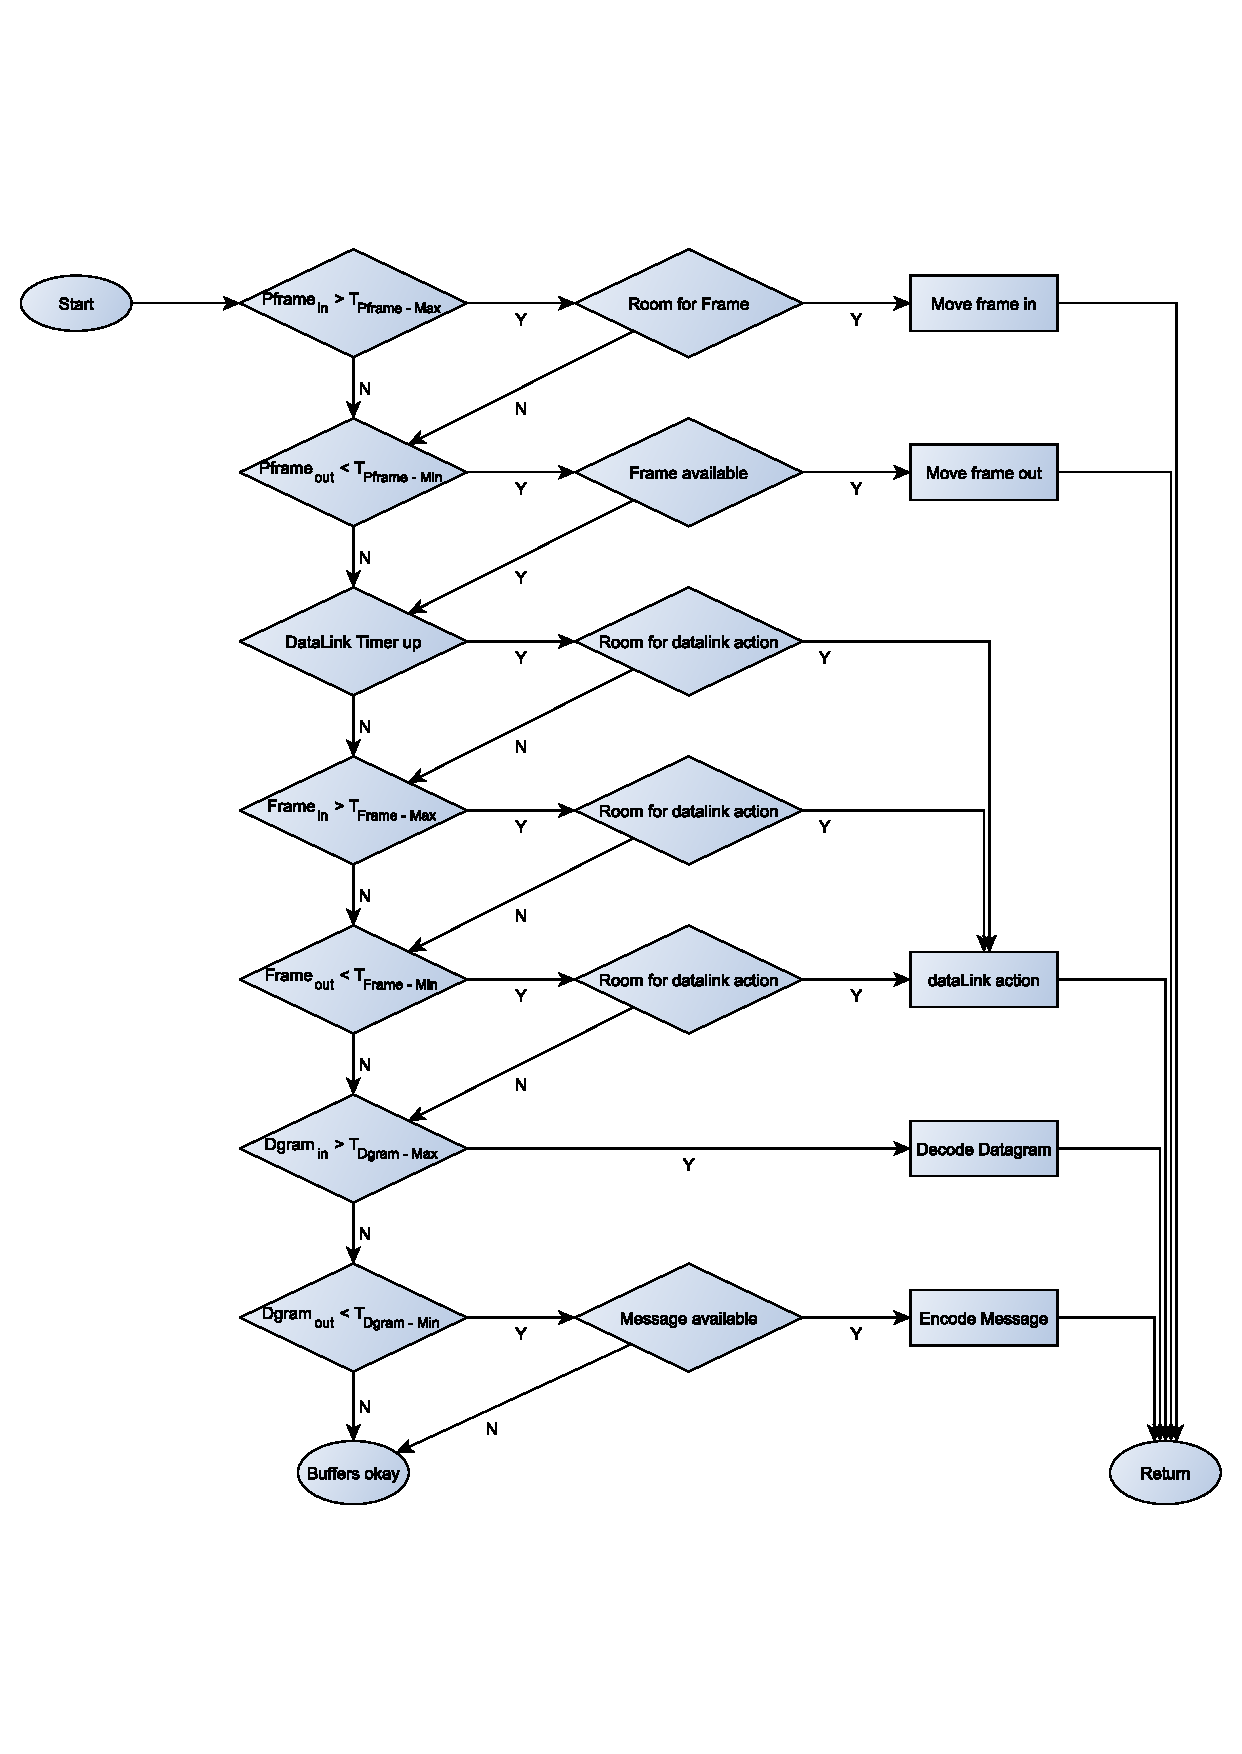
\includegraphics[scale=0.7,trim=0 0 0 0]{backbonePrime.pdf}
	\caption{Backbone primary flow}
	\label{fig:backboneprime}	
	\end{center}
\end{figure}


\begin{figure}[htb]
	\begin{center}
	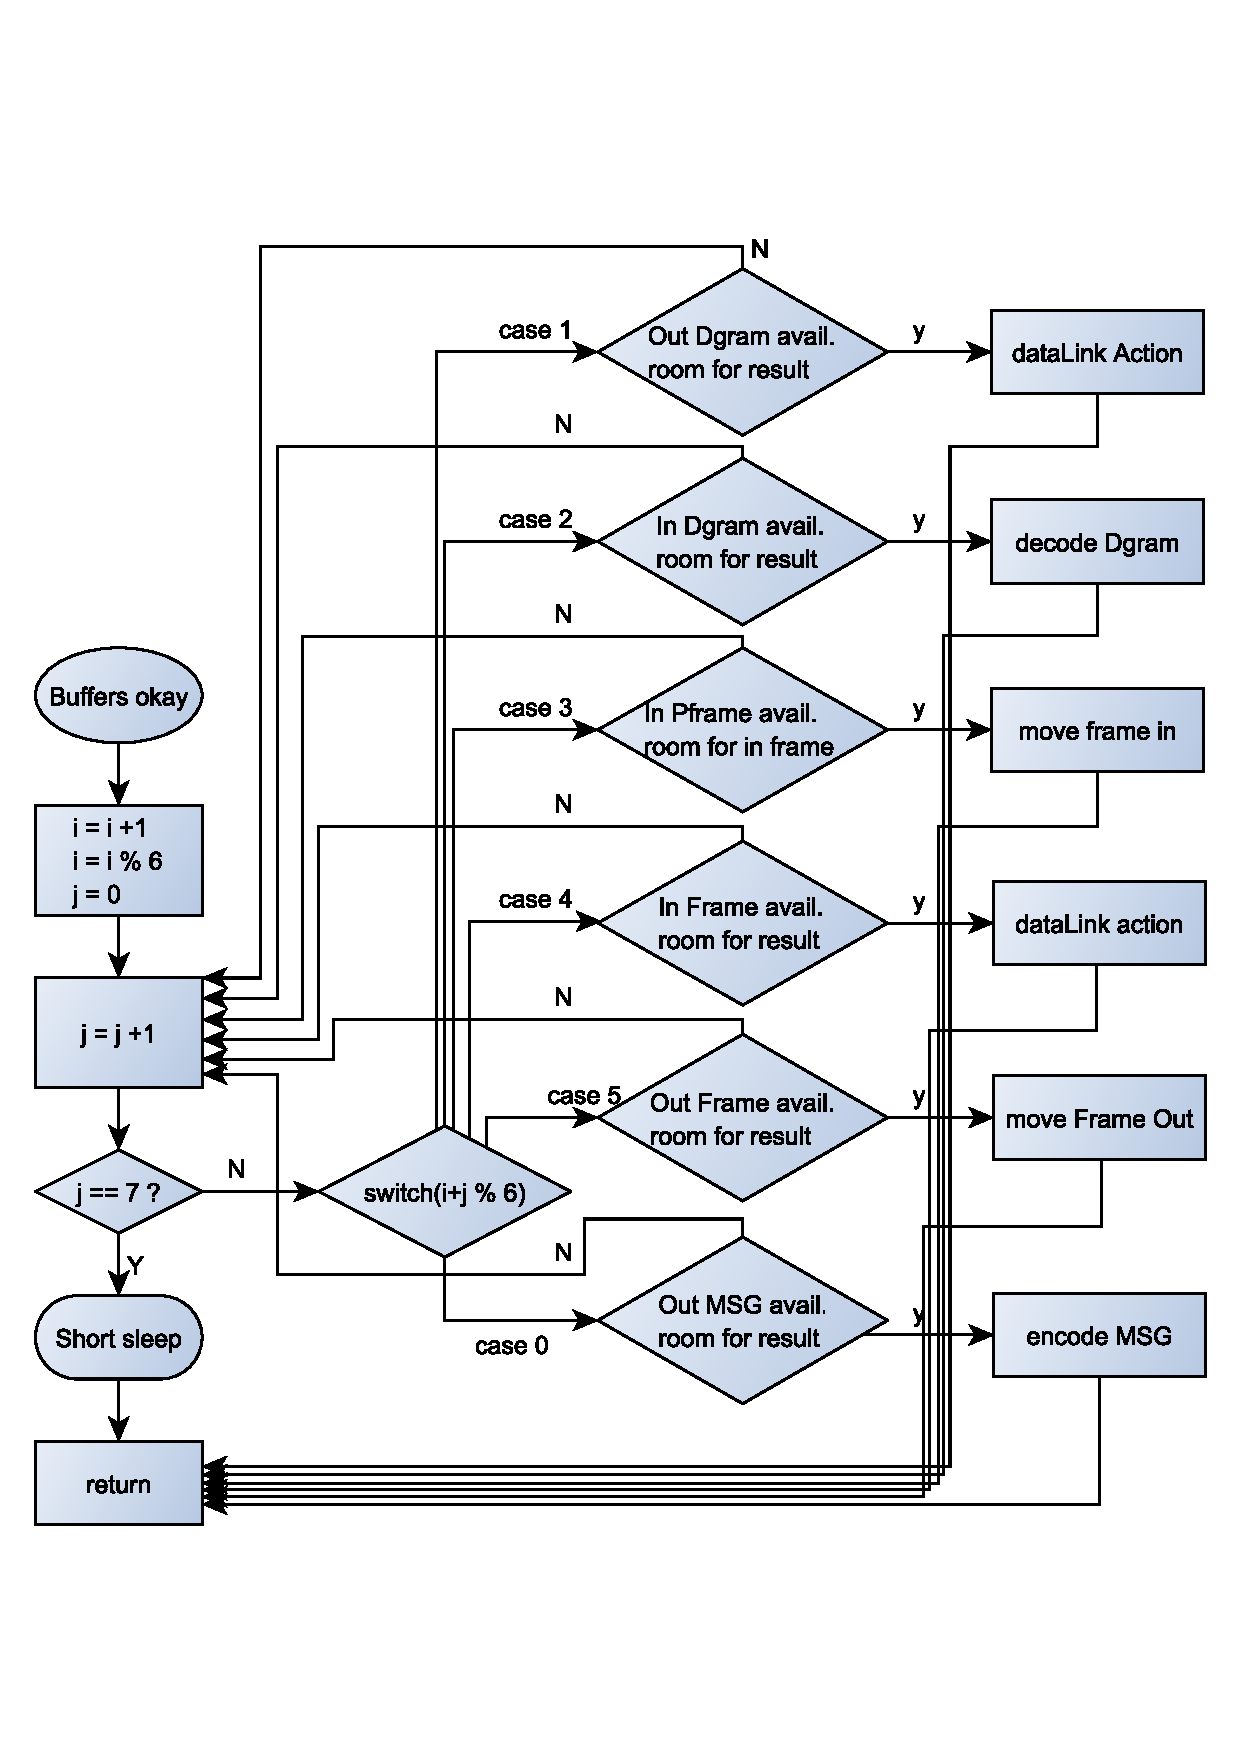
\includegraphics[scale=0.7,trim=0 0 0 0]{backboneGeneral.pdf}
	\caption{Backbone general flow}
	\label{fig:backbonegeneralt}	
	\end{center}
\end{figure}
